\section{Results}\label{sec:results}

Having already described both the apparatus and the method by which your data were acquired, it is now time to present your results.

\begin{figure}[ht]
    \centering
    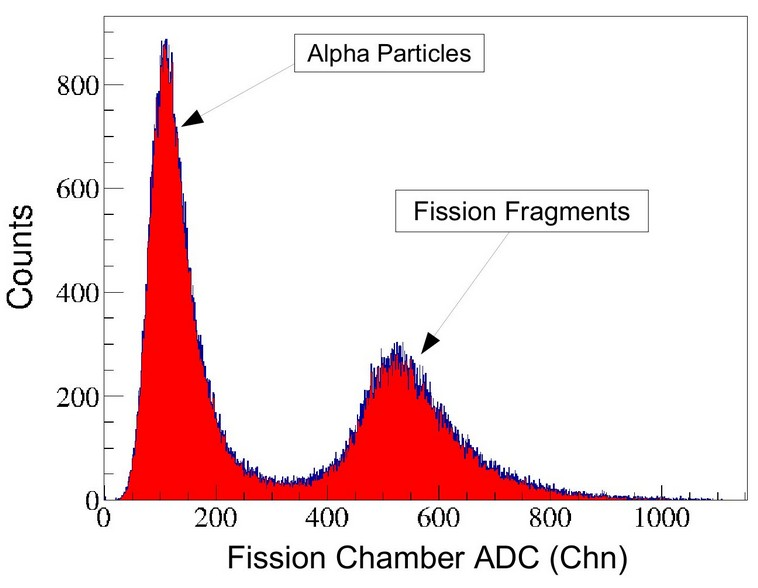
\includegraphics[width=0.8\linewidth]{figures/fission_spectrum.png}
    \caption{\footnotesize The measured energy spectrum in the fission chamber. The separate peaks are from alpha particles emitted in the radioactive decay of $\prescript{238}{}{\text{U}}$, and nuclear fragments created by neutron-induced fission.\cite{Kov_22}}
    \label{fig:fission_spectrum}
\end{figure}

In many experiments, the 'raw data' consist of a measured spectrum of one form or another. In such a case, you should present just one example spectrum, such as the one shown in Fig. \ref{fig:fission_spectrum}. Either on this figure, or in its caption, make note of any important spectral features. The text of your paper should expand on the short description contained in the figure caption.

In other types of experiments, the data consist of a set of measured x-y values. You might have used, for example, a digital voltmeter (DVM) to measure the photocurrent produced by the photoelectric effect when you illuminated a metal surface with a steady light source. The dependent variable is the measured current, while the independent variable is the applied retarding potential. Your measurements would then consist of a number of x-y data points, and these should be shown in your paper. (You may actually have collected several such data sets, but only one set should appear as a figure in the paper. You should, however, mention these additional data in the text.) We show in Fig. \ref{fig:photocurrent} an example plot of a complete x-y data set.

\begin{figure}[ht]
    \centering
    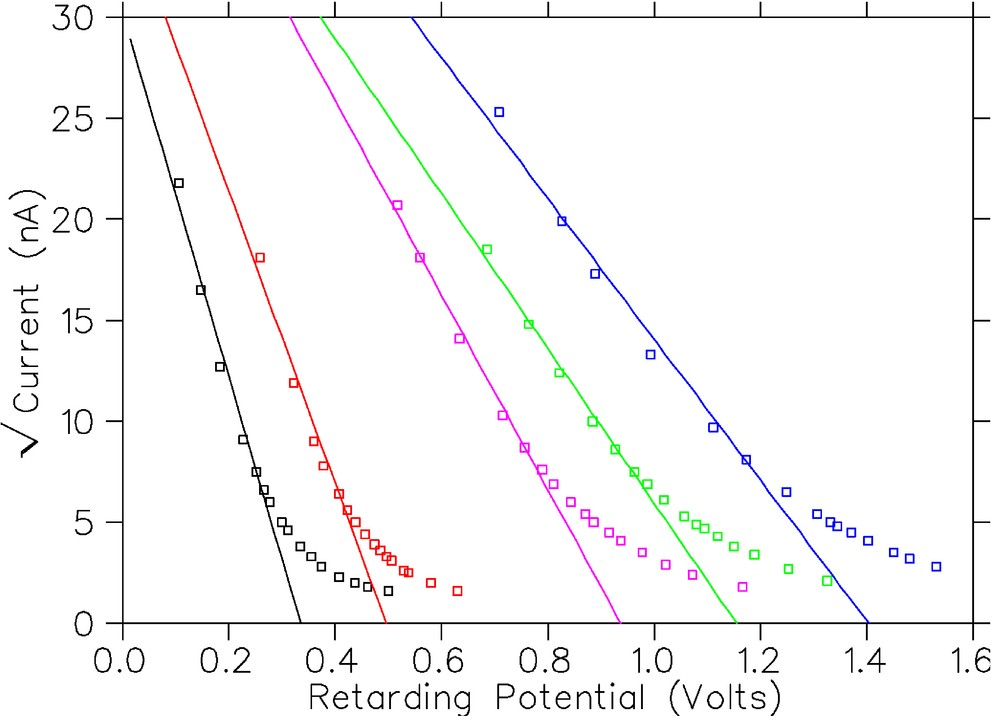
\includegraphics[width=0.5\linewidth]{figures/photocurrent.png}
    \caption{\footnotesize Measured photocurrent as a function of retarding potential. The data sets shown above, reading from left to right, were collected at wavelengths of 577, 546, 436, 405, and 365 nanometers.\cite{Kov_22}}
    \label{fig:photocurrent}
\end{figure}

Notice how the axes on this and our other figures are scaled so as to fill the frame with the measured results. Each axis is labeled with the name of the displayed quantity, and its units. In Python, you can easily add a legend to the figure, providing additional clarity for the reader. Note that error bars are not typically shown on data which are obtained with a DVM.

In addition to showing your unprocessed data in a figure, the Results section will also include a tabulation of the numerical values derived from an analysis of your measurements.

Consider the measurements shown in Fig. 3 as an example. The data collected at each wavelength are fit to a linear function over a range of retarding potentials that extends only up to the 'knee' in the data. These fitted curves are shown overlaid on the data. Using the parameters derived from these fits, we determine the stopping potential at each wavelength, along with the estimated errors. (Recall that you can obtain an estimate of the statistical error of any parameter value from the sample standard deviation derived from several data sets.) Since these stopping voltages are an important result of our experiment, they have been listed in Table \ref{tab:stopping_voltage}.

\begin{table}[htbp]
    \centering
    \begin{tabular}{| c | c |}
        \hline
        $\bm{\lambda}$ \textbf{nm} & $\bm{V_\textbf{stop}}$ \textbf{(Volts)} \\ \hline
        577 & 0.335 (0.034) \\ \hline
        546 & 0.496 (0.050) \\ \hline
        436 & 0.937 (0.094) \\ \hline
        405 & 0.937 (0.094) \\ \hline
        365 & 1.40 (0.14) \\ \hline
    \end{tabular}
    \caption{\footnotesize The fitted stopping voltage at each of the five wavelengths studied. The estimated errors are shown in parentheses. (Note the use of leading zeros.)}
    \label{tab:stopping_voltage}
\end{table}

Finally, in most experiments our overall objective is to determine the numerical value of one or more physical parameters. Usually, these values are determined by fitting our analyzed data and reporting the 'best fit' parameters and their errors. Your paper should include a figure which shows this analysis. That figure should contain both your measured points and the overlaid fitting function. For example: We show in Fig. \ref{fig:index_refraction} the results of a fit of our refractive index measurements at four wavelengths.
\begin{figure}[h]
    \centering
    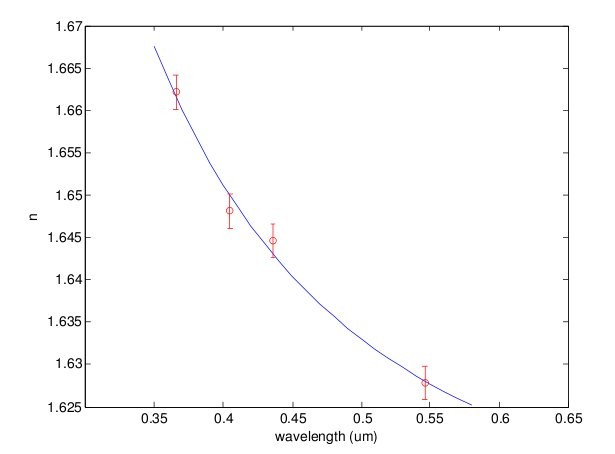
\includegraphics[width=0.9\linewidth]{figures/index_refraction.png}
    \caption{\small The measured index of refraction for flint glass. The curve shows the results of a fit to the form (say) of Eq. (\ref{eq:photoelectric_energy}).\cite{Kov_22}}
    \label{fig:index_refraction}
\end{figure}